\documentclass[12pt]{report}
\usepackage[page,toc]{appendix}
\usepackage[style=ieee]{biblatex}
\addbibresource{references.bib}
\usepackage{enumitem}
\setlist[enumerate]{nosep}
\usepackage{etoolbox}
\usepackage{fancyhdr}
\usepackage{float}
\usepackage{fontspec}
\usepackage[letterpaper,hmargin={47.5mm,17.5mm},top=64.0mm,bottom=25.4mm]{geometry}
\usepackage{indentfirst}
\usepackage{listings}
\usepackage{microtype}
\usepackage{multirow}
\usepackage{setspace}
\usepackage{tabularx}
\usepackage[explicit]{titlesec}
\usepackage{tocbibind}
\usepackage{wallpaper}

\newcommand{\authora}{
    Melba Dominique B. Castorico %
}
\newcommand{\authorb}{
    Basil Eric Rabi %
}
\newcommand{\codesnippet}[2]{
\begin{scriptsize}
\lstinputlisting[#1]{#2}
\end{scriptsize}
}
\newcommand{\eg}{\emph{e.g.}}
\newcommand{\hypothesis}[3]{
\noindent \textbf{Research Question:}
\par#1
\begin{quotation}
    \noindent \textbf{Null Hypothesis ($H_o$)}:
    \par#2

    \noindent \textbf{Alternative Hypothesis ($H_a$)}:
    \par#3
\end{quotation}
}


\newcommand{\thetitle}{Development of a Multi-Dimensional Pit Optimization System for Strategic Planning in Surface Mines}

\usepackage[hidelinks]{hyperref}
\hypersetup{
    pdfborder  = {0 0 0},
    pdfinfo    = {
        Title    = {\thetitle},
        Subject  = {Mine Economics},
        Author   = {\authora and \authorb},
        Keywords = {Optimization, Mining, Mine Economics, Strategic Mine Planning}
    }
}

\addtolength{\headwidth}{15pt}
\doublespacing
\renewcommand{\contentsname}{TABLE OF CONTENTS}
\renewcommand{\headrulewidth}{0pt}
\setmainfont[Mapping=tex-text-ms]{XITS}
%\setmainfont[Mapping=tex-text-ms]{Times New Roman} % TODO: set up Times New Roman in github workflow
\setmonofont{DejaVu Sans Mono}
\setlength{\headheight}{15pt}
\setlength{\parindent}{12.7mm}
\setcounter{secnumdepth}{3}
\titleformat{\chapter}[block]{\bfseries\centering}{}{0em}{#1}
\titlespacing{\chapter}{0pt}{-30pt}{0pt}
\titlespacing{\section}{0pt}{0pt}{0pt}
\titlespacing{\subsection}{0pt}{0pt}{0pt}
\titlespacing{\subsubsection}{0pt}{0pt}{0pt}

\begin{document}

\ULCornerWallPaper{1}{spus.pdf}
\pagenumbering{roman}
\addcontentsline{toc}{chapter}{TITLE PAGE}
\thispagestyle{empty}

\begin{center}

\textbf{\MakeUppercase{\thetitle}}

\vspace{1.5cm}
A Thesis Proposal Presented to \\
The Faculty of the College of Engineering \\
St. Paul University Surigao \\
Surigao City

\vfill

In Partial Fulfillment \\
of the Requirements for the Degree \\
BACHELOR OF SCIENCE IN MINING ENGINEERING

\vspace{1cm}
By:

\vspace{1cm}
\textbf{\authora} \\

\vspace{1cm}
November 2023

\end{center}

\fancypagestyle{plain}{
    \fancyhead{}
    \fancyfoot{}
    \fancyhead[R]{\thepage}
}

\pagestyle{fancy}
\fancyhead{}
\fancyfoot{}
\fancyhead[R]{\thepage}

\tableofcontents

\titleformat{\chapter}[block]{\bfseries\centering}{CHAPTER \thechapter\\#1}{0em}{}
\titleformat{\section}[block]{\bfseries\centering}{\MakeUppercase{#1}}{0em}{}
\titleformat{\subsection}[block]{\bfseries}{#1}{0em}{}
\titleformat{\subsubsection}[block]{}{\emph{#1}}{0em}{}

\chapter{THE PROBLEM AND ITS BACKGROUND}

\pagenumbering{arabic}

\section{Introduction}

\subsection{Mineral Reserves and Optimized Strategic Plans for Surface Mines}

Mine planning software that are utilized in scoping, feasibility, life-of-mine scheduling and in the ongoing re-evaluation of mine plans through production phase.
Accurate evaluation of financial viability of the mineral deposit and development, then determination of the optimal long term strategic mine plan and schedule to extract the full value of that deposit over the life of the mine. 
However, the Algorithm that analysis the conditions for scheduling includes strategic scheduling, detailed cost, price and recovery modeling, multiple scenario analysis, blending, cut-off and simultaneous stockpile optimization and failed to consider the open area for extraction of ore as mandate by existing guidelines. 
Thus, full potential of mine project is not fully attained.
Simultaneous mine production and mine rehabilitation is the major focus on the development of this algorithm for attainment of the optimum life-of-mine.

\subsubsection{Optimized Economics}

Economic optimization entails striving to acquire the best from economy in terms of profits, production, and utility.
In entails maximizing the objective functions which contribute towards the best economic outcome.

\subsubsection{Good Governance and Environmental Compliance}

Environmental resources is essential in economic advancement and the improvement of society's quality of life, and strong environmental governance in important in achieving goals in sustainable way. 
Mining assumes governance as key to the environment and, as a consequence, to the business.
The development of the algorithm that will provide the full potential of mine project without compromising the environment is a sustainable attainment of economic growth.

\subsubsection{Open Area Restriction}
In Surface mining, the maximum area for the extraction of ore at any one time shall be dependent on the scale of the mining operation.
For projects that have processing plants, the maximum disturbed area for extraction is one hundred sixty-two (162) hectares or two (2) meridional blocks (DAO 2018-19) \cite{DAO2018-19}.
Temporary revegetation or progressive rehabilitation shall be implemented immediately on disturbed area exceeding the maximum disturbed area.

\subsection{Auditability}

Auditability of the source code is significant in order to determine how the algorithm handled the data and how it analysis it and ensure that it is not bias. 

\section{Conceptual Framework of the Study}

This study aims develop a life of mine optimizer for surface mines or LOMOPTIM for short..
There will be 3 major milestones in the development cycle of the study as illustrated in Figure~\ref{fig:conceptual_framework}.

\begin{figure}[p]
    \centering
    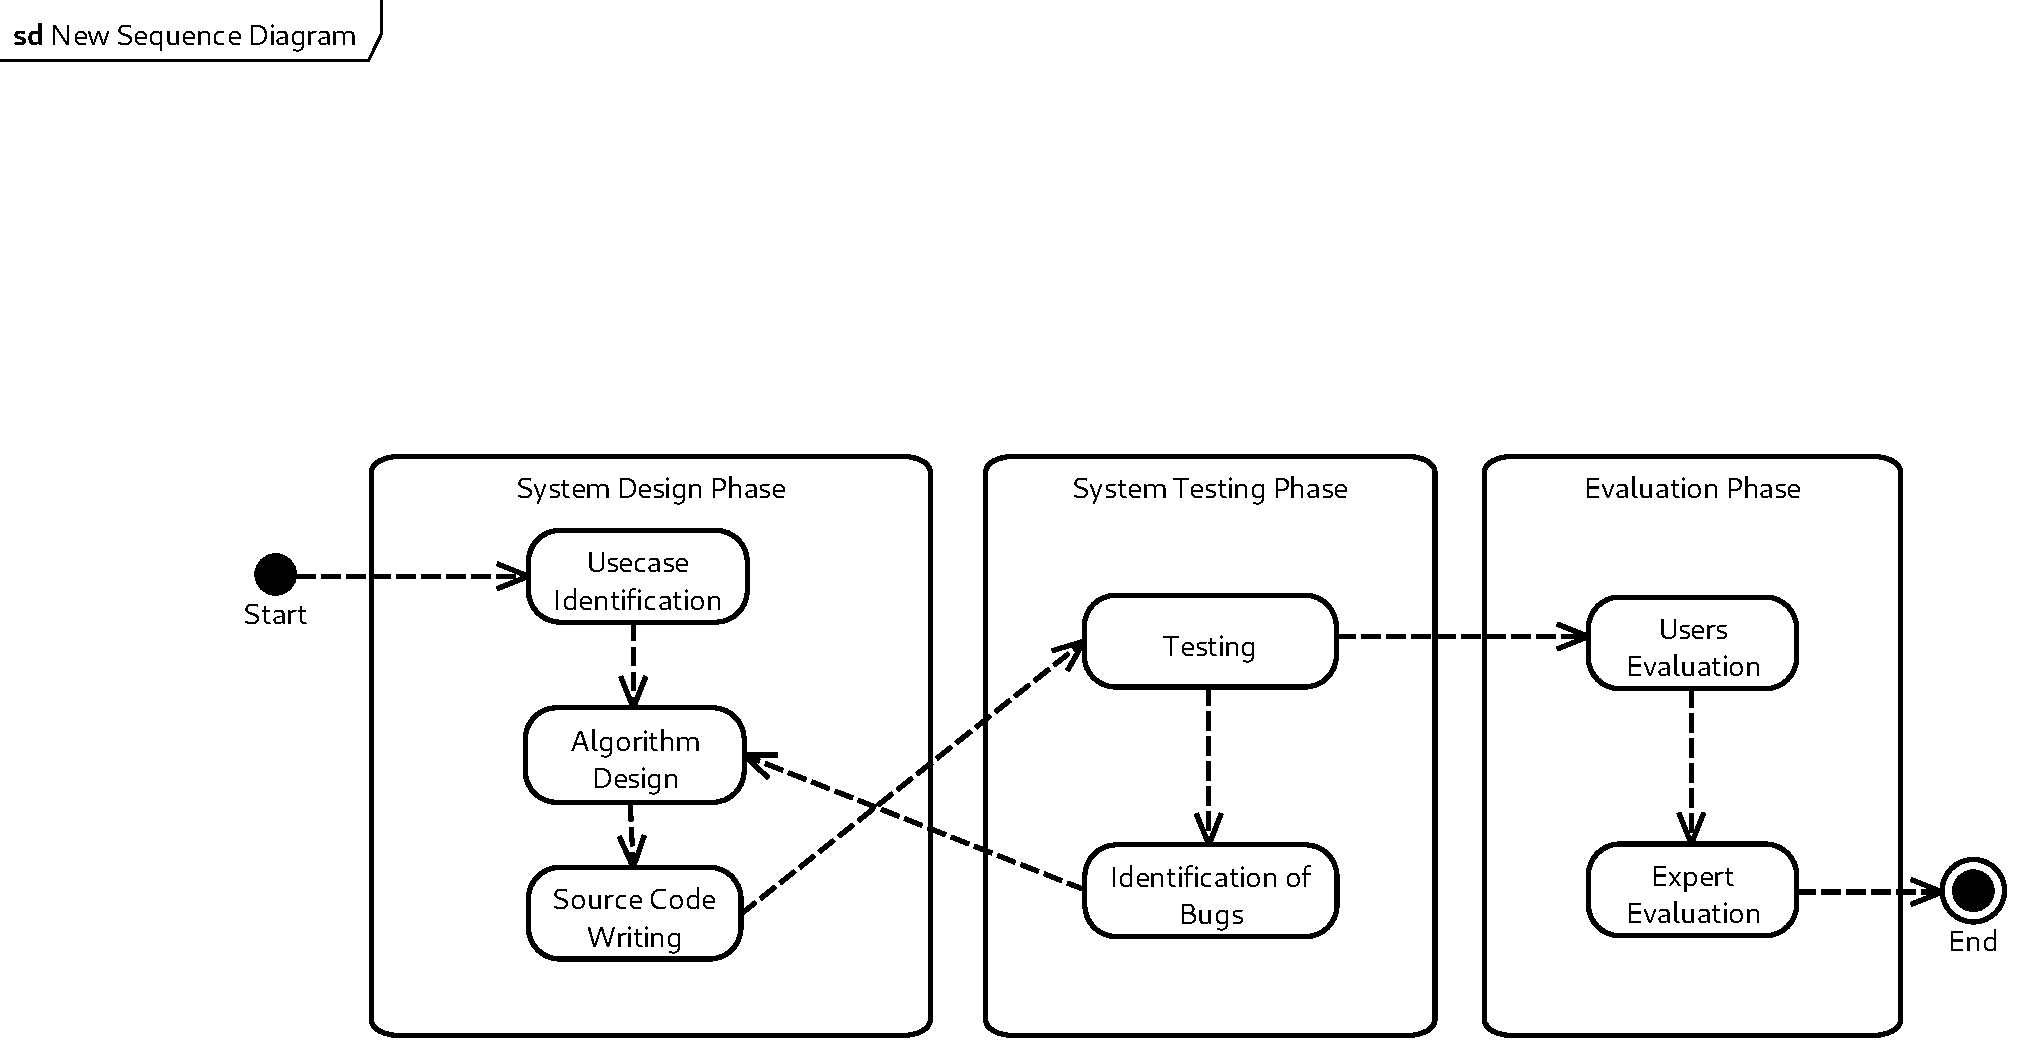
\includegraphics[clip, trim=30mm 2mm 2mm 33mm, width=\linewidth]{img/conceptual_framework.pdf}
    \caption{Development cycle of LOMOPTIM.}
    \label{fig:conceptual_framework}
\end{figure}

The first part is the system design phase which will include use case identification, algorithm design and source code writing.
Once the design phase is done, the next stage will be the system testing phase wherein the functionality of LOMOPTIM is as expected and no bugs are present.
Should bugs be identified, the algorithm and the source code will be modified.
The final part of the study will be the evaluation phase wherein LOMOPTIM will be tested by the strategic mine planners and other technical experts.

\section{Statement of the Problem}

\begin{enumerate}
    \item What is the status of the current system for strategic mine planning in terms of
        \begin{enumerate}
            \item Processing time in achieving the highest net present value
            \item Achieving the throughput requirement per product
            \item Achieving the yearly slices which complies to the environmental requirements stipulated in DAO 2018-19
        \end{enumerate}
    \item How is the system developed in relation to
            \begin{enumerate}
                \item Software stack selection
                \item Current tools used by the company
                \item End-user's requirements
            \end{enumerate}
    \item How does the new system compare to the existing system for strategic mine planning?
    \item What is the evaluation of the system by the experts and users in terms of
        \begin{enumerate}
            \item Efficiency
            \item User's experience
        \end{enumerate}
\end{enumerate}

\section{Significance of the Study}

The objective of the study is to produce a working application which will determine an economically optimum yearly mining sequence from an arbitrary start up to the end of the mine life while prioritizing sub-optimal restrictions like a minimum annual product throughput and a maximum open area at the end of every year.


\subsection{Surface Mine Planners}

This study makes it possible to create a repeatable and auditable process in creating life-of-mine plans.
The development of a system for a Life of Mine optimizer for surface mines in which mine planners will participate and contribute for the inputs and determination of the optimal condition. 
This study aims to provides a strategic mining sequence with confidence and a non-bias result that will suffice the needs and expectation for a mining project.

\subsection{Mining Community}

Implementation of optimal system in planning for surface mines will benefit the mining community as this will simplify the compliance on restriction for open areas for surface mine. 
Maximizing the recovery while prioritizing the implementation of good governance and environmental compliance.
Establishment of relationship between environmental stewardship and economic success for the success of a mining project.
By minimizing the ecological footprint and enhancing operational efficiency, mining operations can achieve balance that not only benefits the environment but also ensure sustainable and economically viable practices over the long term.

\subsection{The host Mining Community}

This study is in-line with the goal of good governance of the mining industry through the prioritization of legal compliance while also taking in consideration the optimum economics.

\subsection{Academe}

Since the systematic approach of Life of mine optimization will readily available, it will be easier for Academe and other organizations to assess what mining engineering students needs to be taught in order to generate graduates who are qualified and equipped.

\section{Scope and Limitation of the Study}

The development of the application focuses only on the case of Taganito Mining Coporation (TMC) which has a partner plant using the High Pressure Acid Leach technology.
This plant requires a consistent throughput of limonite ore while TMC's mine product is saprolite ore.
Thus, this study will only account for two products for the mine optimization: limonite and saprolite.

In addition, the programming side of the application will be done in Fedora Linux \cite{fedora} since the programming toolkits such as the C++ compilers, Qt libraries, and data processing tools such as Postgresql \cite{postgres} and PostGIS \cite{postgis} are readily available.

\chapter{REVIEW OF RELATED LITERATURE}

\section{Surface Mining}

The surface mining method is the most common method in mining due to its cost effectiveness but at the same time, it's visual and environmental impacts are the most conspicuous such as deforestation, dust generation, and surface run-offs.
Thus, it is very imperative to minimize to open area in a surface mine in order to also keep the these impacts at its minimum.
In this research, one dimension which will be considered during mine optimization is not exceeding the allowable open area at any given time in order to comply with DAO 2018-19 and minimize the environmental impacts.

\section{Taganito Mine and the Laterite Profile}

The mine project which will host this research is Taganito Mine located in Taganito, Claver, Surigao del Norte.
Taganito Mine sits on top of a nickeliferous laterite deposit which produces two distinct products: limonite and saprolite.
The nickeliferous laterite deposit is produced from the chemical weathring process of ultramafic rocks such as peridotite and dunites.
In a mature laterite profile, the layers arranged in the following order from bottom-up: bedrock, saprolite zone, and limonite zone.
The bedrock layer is comprised by serpentinized dunites and peridotites with some notable joints and fractures caused by uplifiting.
The saprolite zone is where the most nickel is enriched through precipitation during partial dissolution of nickel during weathering.
Due to the enrichment of nickel in the saprolite, saprolite ore with sufficient nickel content can be used as ore feed for ferronickel smelting plants.
The most chemically altered portion in the laterite profile is the limonite zone.
Most magnesium and silica are removed in the limonite zone due to weathering while the non-mobile elements such as iron, aluminum, chromium are retained as residue.
Thus, the limonite zone is usually characterized by high iron and chromium content.
Because of this, the ore from limonite can be used as ore feed for iron smelting plants and a source for chromite.
In the case of Taganito Mine, the limonite is exclusively sold to a High Pressure Acid Leaching Plant as an ore feed for the production of Ni-Co mixed sulfide.

\section{Existing Tools and Algoritms}

\subsection{Lerch-Grossman}

The most common algoritm used in mine optimization is the algorithm described by Helmut Lerch and Ingo Grossman.
This can be illustrated with each mine block with both downward force (cost) and upward force (revenue value).
The objective of this algorithm is to maximize the total upward force without accounting for the mining sequence \cite{IMS}.

\subsection{Pseudoflow}

A variation of the Lerch-Grossman algorithm (LG) which adapted a network analysis of directed graphs and spanning trees is called the pseudoflow.
Although there are also lots of variations of this algoritm, the best variants chosen in most literatures are lowest label and highest label methods \cite{pseudoflow}.

\subsection{GEOVIA Whittle}

GEOVIA Whittle is proprietary strategic mine planning tool which is commonly used in the Phillipines by various surface mines.
This application implements the abovementioned algorithms in mine optimization, Lerch-Grossman and Pseudoflow, while maximizing the Net Present Value of the generated annual pit shells \cite{whittle}.

\subsection{Limitations of GEOVIA Whittle and Its Algorithms}

Although commonly used in the Phillipines, GEOVIA Whittle at present cannot conform to the recent developments of laws related to mining such as the DAO 2018-19 \cite{DAO2018-19} which limits the open area of all mines since GEOVIA Whittle focuses only on addressing engineering design constraints and economic optimization.
In addition, GEOVIA Whittle is able to consider a minimum extraction limit but cannot set a minimum production limit for a specific product.
In the present mineral prices, saprolite ore is more valuable than limonite ore so GEOVIA Whittle will prioritize saprolite ore in the annual production instead of the limonite ore.
However, in the case of Taganito Mine where a minimum production of limonite ore is required to sustain a High Pressure Acid Leach plant, using GEOVIA Whittle will only a produce an unacceptable yearly production.

\section{Development Tools}

\subsection{C++}

The programming language to be used in the development of LOMOPTIM will be C++.
This a high level language which applies object-oriented programming for easier data abstraction.
It also implements easier memory management through the use smart pointers and efficient use of multi-threaded machines through threading and mutual exclusions \cite{cpp}.

\subsection{Qt}

In the creation of the graphical user interface of LOMOPTIM, the C++ toolkit called Qt will be used.
Qt is a graphical toolkit built for C++ which already contains a lot of libraries of graphical elements.
Included in this toolkit is the graphical designer which will allow the reaserchers to design an interface without writing a single line of code \cite{qt}.

\chapter{METHODS}

\section{Research Design}

This study aims to design and develop an application which will mainly comprise of systems designing and writing of software components.
During the initial part of the research, the descriptive-developmental design will be applied in order to understand the existing system used in strategic mine planning and identify the gaps.
During the next phase of the research which is the system design phase,, a multi-phase iterative approach as discussed by Leedy and Ormrod will be applied.
This research design is used commonly in design-based research wherein the researchers apply existing knowledge to create more effective systems \cite{MixedMethod}.

\section{Respondents}

LOMOPTIM will be tested mostly by the mine planners in Taganito Mine and possibly other mine planners of other operating mines of Nickel Asia Corporation.
The researchers will formulate a method of preparing the sample data input.
The output of LOPTIM will then be compared with in GEOVIA Whittle by the participating mine planners.

\section{Methodology}

\subsection{System Design}

\subsubsection{Use Case}

The basic use case \cite{usecase} of LOMOPTIM is illustrated in Figure~\ref{fig:usecase}.
The user will input both the block model file and various engineering parameters which will be enumerated further during the study.
Some identified parameters are bench width, bench height, bench slope, extraction limit in wet metric tons, maximum open areas in hectares, and minimum extt tonnage
After completion of inputs, the user can run the algorithm which will output the yearly pit shells and the yearly production details which should include tonnages and grades.

\begin{figure}[p]
    \centering
    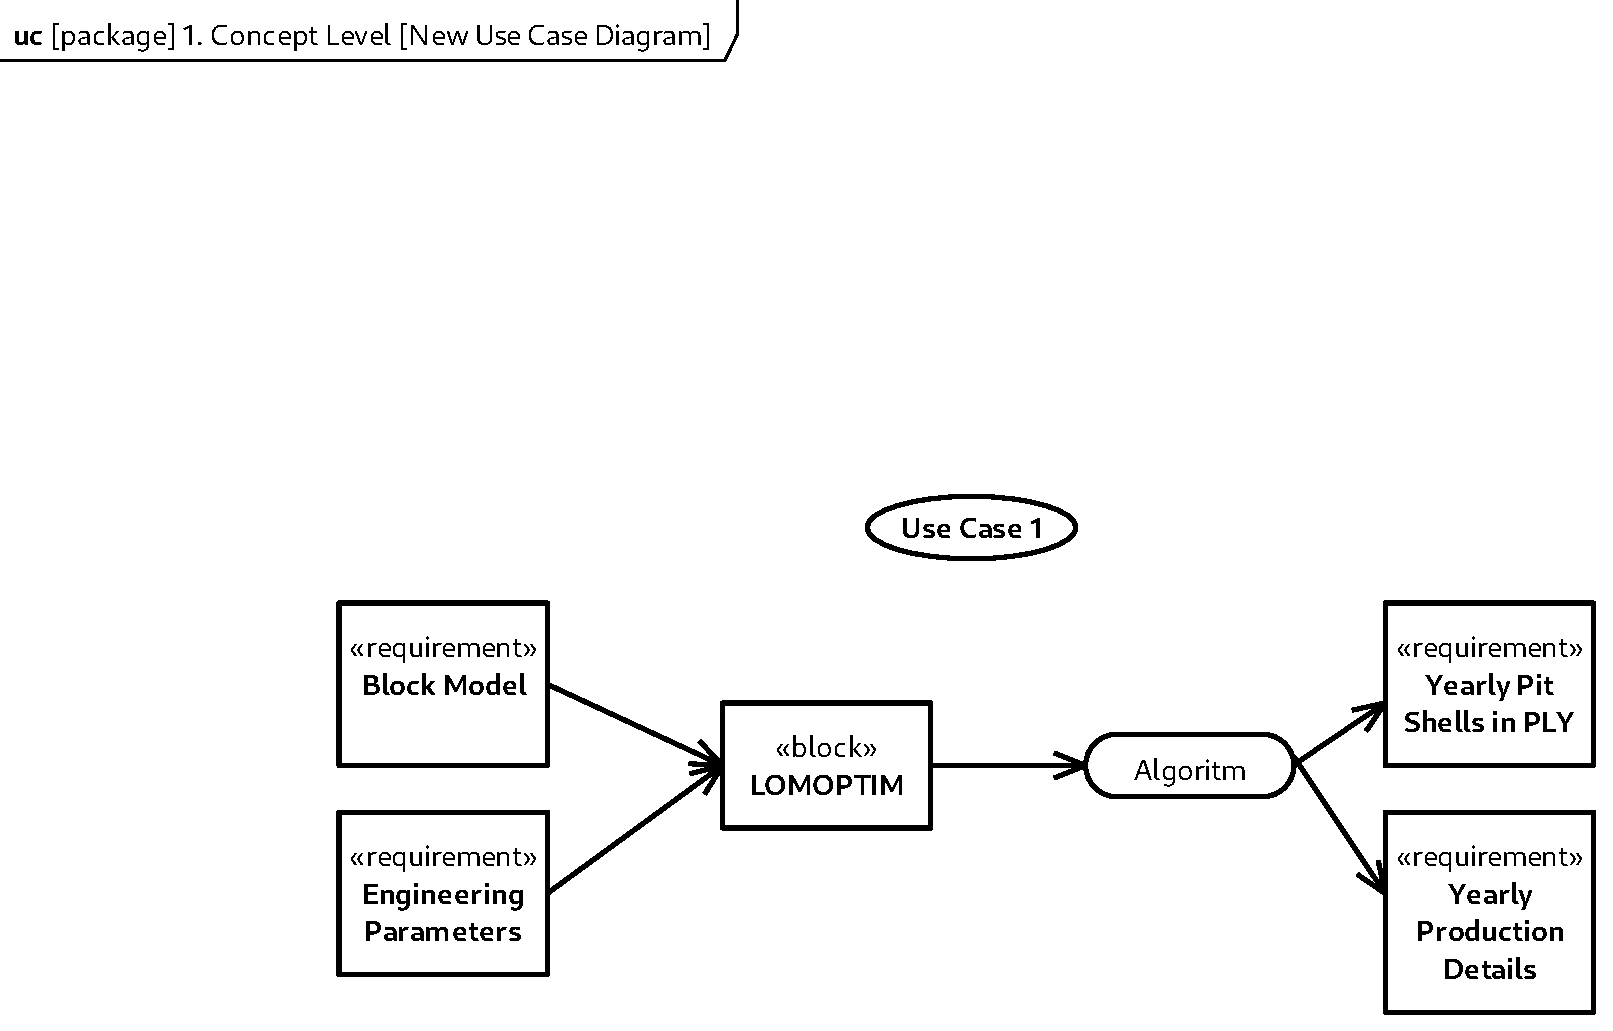
\includegraphics[clip, trim=15mm 0 0 12mm, width=\linewidth]{img/usecase.pdf}
    \caption{Initial use case of LOMOPTIM.}
    \label{fig:usecase}
\end{figure}

\subsubsection{File Structures}

The block model input will be composed of 3 comma-delimited files (CSV) which just contain ASCII texts.
The first CSV file will be comprised by the collar data of the block model which will contain the 3D coordinates.
The second CSV file will be comprised by the block model itself which will contain the chemical characteristics of block down each collar with its quantified extraction cost and revenue values.
The extraction cost and revenue values will be prepared beforehand while each block may have different rock types at varying compenents.
The last CSV file will contain the rock type or product type along with their corresponding bulk densities and moisture contents.

\subsubsection{Algorithm}

The algorithm to be used in LOMOPTIM will be a brute-force approach wherein each mining sequence will be explored if it conforms to the engineering constraint inputted by the user.
All iteration will be predetermined using permutation included in the C++ standard library through parallel computation (threading).
Each finished iteration which conforms to the engineering constraints and also results to the a higher net present value will be saved through mutual exclusion to prevent race conditions of each iteration.


\subsection{Source Code Writing}

The source code of LOMOPTIM will be solely written in C++ \cite{cpp} in the development environment called Qt Creator which is part of the Qt toolkit \cite{qt}.

\section{Instruments}

During the development of LOMOPTIM, free and open source tools will be used as discussed in the review of related literature.

In the method of qualitative evaluation, a similar method based on the ER Mine Tracer research design will be applied wherein the researchers of the said study used survey to qualitatively evaluate ER Mine Tracer's functionality and efficiency \cite{ERMineTracer}.

In the preparation of data, data management tools such as PostreSQL \cite{postgres}, PostGIS \cite{postgis}, and R \cite{R} will be used.

\section{Data Gathering Procedure}

\subsection{Quantitative Data}

The efficiency and effectiveness of LOMOPTIM will be evaluated in terms of compliance with the input restrictions and processing time.

\subsection{Qualitative Data}

Qualitative data will be collected through the use of questionnaires to the potential users, engineers, and technology experts if available.
Each question will be have a corresponding point system similar to the Liker 4-point scale \cite{Likert}.

\section{Data Analysis}

The performance of LOMOPTIM will be compared to Whittle which is the existing system used by TMC.
The researchers will be using R version 4.3 \cite{R} to analyze the quantitative data.

Questionnaire surveys with qualitative information will be distributed to Strategic Mine Planners, IT Experts, Computer Engineers and other experts on this topic in order to collect data that are qualitative in nature.

The result of the surveys and the collected quantitative data will be used by the researchers to determine if LOMOPTIM meets the user's requirements, meets the standard's of the technical experts, and does not have any technical limitations that might hinder its adoption.

\chapter{RESULTS AND DISCUSSION}

Surface Mines has a lot of mandated laws and guidelines to follow that limits the full potential of current Mine Planning Software in generating Optimal Life of Mine plans.
This leads to the development of an algorithm that would suffice the requirements to attain the most profitable and sustainable Mining Project. 
General workflow of the algorithm is shown in Figure~\ref{fig:PFLomoptim}.

\begin{figure}[p]
    \centering
    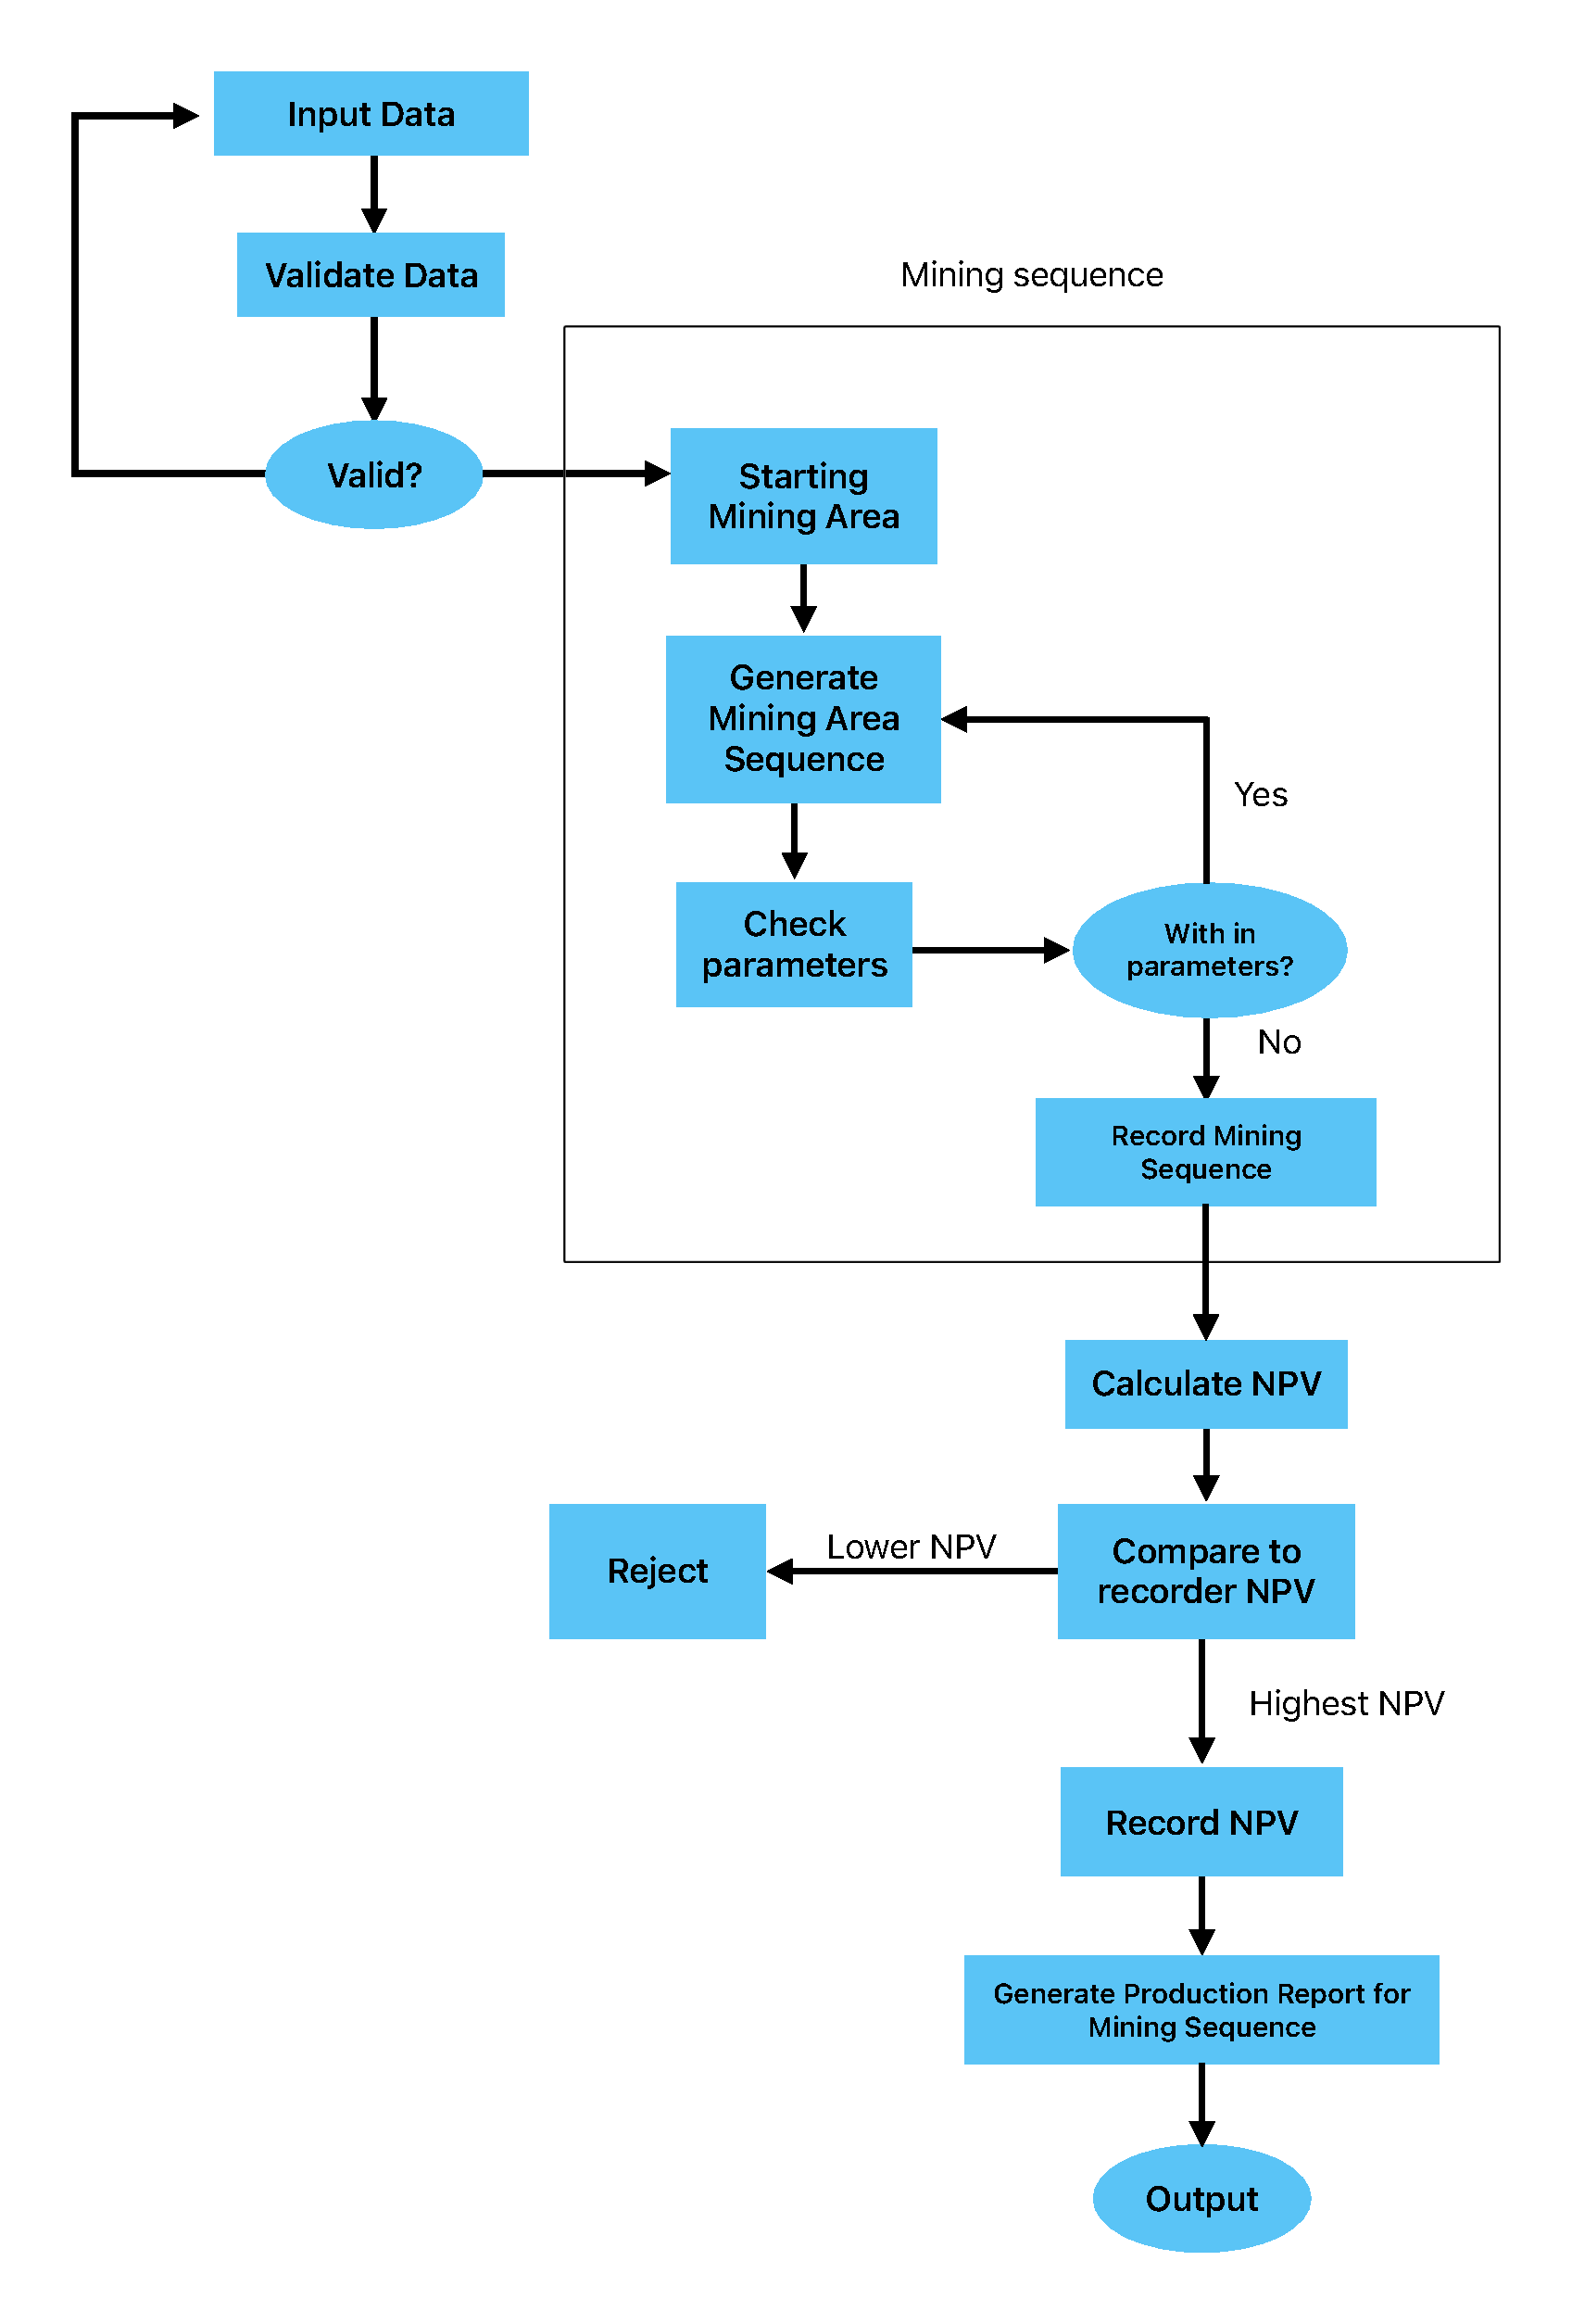
\includegraphics[width=4in,height=7in]{img/PFLomoptim.pdf}
    \caption{High level flow of LOMOPTIM algorithm.}
    \label{fig:PFLomoptim}
\end{figure}

\section{Input Data}

To run the algorithm, the user must specify the data requirements: Block model and Engineering Parameters.
The Block model is the collection of several mining area, each contains specific commodity content and corresponding revenue. 
It also contain the geological characteristic of the mining project. In which the objective of the development of this algorithm is to determine the most profitable sequence of mining the area, considering the various predetermined parameters. By optimizing the revenue potential and specific constraints, the algorithm aims to maximize the profitability of the mining project. 
This is designed for efficient resource allocation and enhance revenue generation, and improve the overall operational effectiveness in resource extraction.

\section{Data Validation}

The algorithm needs to verify that the input block model data contains the necessary attributes and the predefined parameters are within the acceptable ranges. 
Otherwise, the algorithm prompts the user to rectify the error by entering a valid data.
This is done to eliminate errors in generating the Optimal Mining Sequence.

\section{Generation of Mining Sequence}

Multiple Mining sequence is generated for the purpose of determining all the possible outcome of a mining project. 
The algorithm continues to generate the sequence until it encounters the point where the sequence is no longer valid according to the predetermined parameters. 
This iterative process will continue until all possible mining sequence has been considered.

\section{Optimal Net Present Value}

Each Mining Sequence generated in the algorithm has a corresponding production details such as the tonnages, commodities and revenues. 
These details can be used to calculate the Net Present Value (NPV), a fundamental measure used in assessing the profitability of a Mining Project. 
NPV computation involves discounting the expected future revenues of the mining sequence to their present value given to a certain discount rate. 
This methods enables the comparison of revenues generated over the projects duration in present-day term. 
NPV is computed by: 

\begin{figure}[h]
    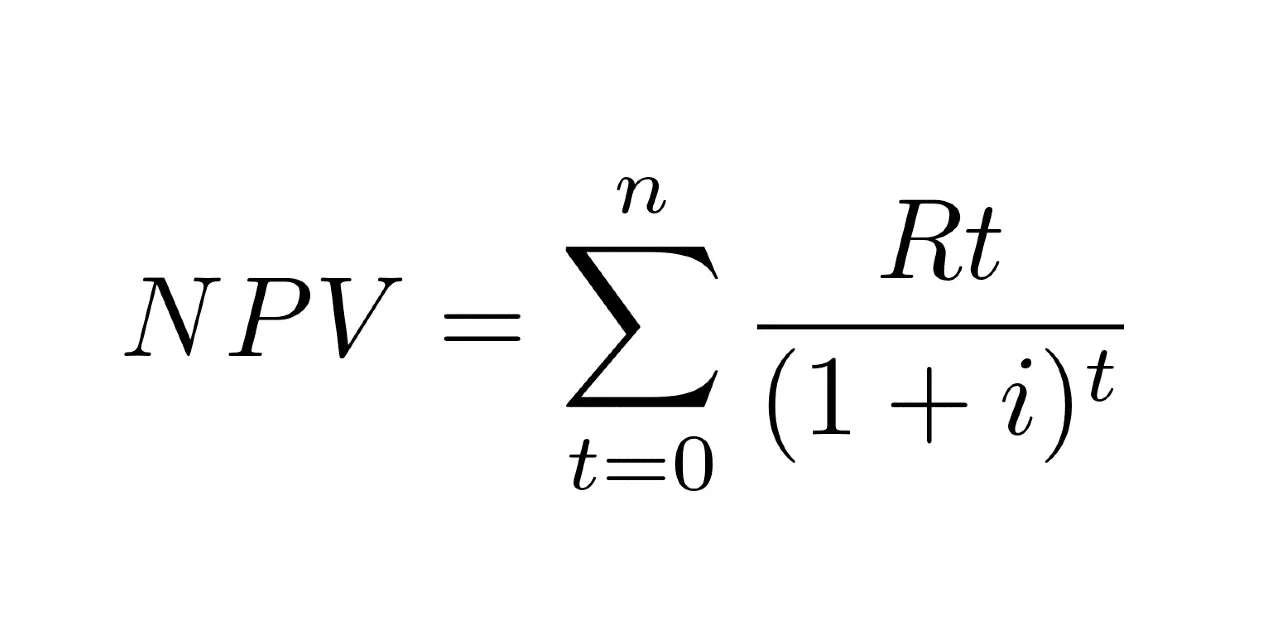
\includegraphics[width=1.5in]{img/NPV}
\end{figure}

\begin{tabular}{@{}l@{ : }l}[h]
 where\\
  Rt & Net cash inflow/ revenue during a single period, t \\
  i & Discount rate\\
  T & Number of timer periods \\
  \end{tabular}
  
\subsection{NPV Calculation for Individual Mining Area}

Every resulting Mining Sequence is comprise with multiple number of Mining Area. 
The calculation of NPV is based one the revenue by series of mining area. 

\subsection{Discounting Cash Flows to Present Value}

Once the expected revenue for each mining area are determine, the algorithm discounts these future revenue to their present value using the NPV method.
The discounting process adjusts the value of future revenue to reflect their worth the the present day term, accounting for the value of money and the project’s specific discount rate.

\subsection{Summation of NPV}

After computing the NPV for each mining area within the mining sequence, the algorithm sumps up these NPVs to obtain the total NPV for the entire mining sequence.
By summing up the NPVs across the mining areas, the algorithm evaluates the profitability of the mining sequence, considering the combined revenue potential.

\section{Selection of the Optimal Mining Sequence}

The summation of NPVs per Mining Sequence is noted and compared to the recorded NPV.
The mining sequence with the highest total NPV represents the most profitable and sustainable life of mine plans among the options considered.
The Optimal Mining Sequence will be extracted in form of production report and in yearly pit shell.

\titleformat{\chapter}[block]{\bfseries\centering}{}{0em}{#1}
\printbibliography[
    title = {REFERENCES},
    heading = bibintoc
]

\begin{appendices}

\chapter{SOURCE CODE}

\section{\lstinline{blockmodel.cpp}}
\codesnippet{language=C++,breaklines,showstringspaces=false}{sourcecode/blockmodel.cpp}

\section{\lstinline{blockmodel.h}}
\codesnippet{language=C++,breaklines,showstringspaces=false}{sourcecode/blockmodel.h}

\section{\lstinline{boost.h}}
\codesnippet{language=C++,breaklines,showstringspaces=false}{sourcecode/boost.h}

\section{\lstinline{main.cpp}}
\codesnippet{language=C++,breaklines,showstringspaces=false}{sourcecode/main.cpp}

\section{\lstinline{mainwindow.cpp}}
\codesnippet{language=C++,breaklines,showstringspaces=false}{sourcecode/mainwindow.cpp}

\section{\lstinline{mainwindow.h}}
\codesnippet{language=C++,breaklines,showstringspaces=false}{sourcecode/mainwindow.h}

\section{\lstinline{mainwindow.ui}}
\codesnippet{language=C++,breaklines,showstringspaces=false}{sourcecode/mainwindow.ui}

\end{appendices}

\newgeometry{hmargin={47.5mm,20mm},top=64.0mm,bottom=25.4mm}
\setlength{\parindent}{0mm}

\begin{spacing}{1.55}

\chapter*{CURRICULUM VITAE}
\addcontentsline{toc}{chapter}{CURRICULUM VITAE}

\begin{tabularx}{\linewidth}{@{}lXr}
    \MakeUppercase{\authora} && \multirow{3}{*}{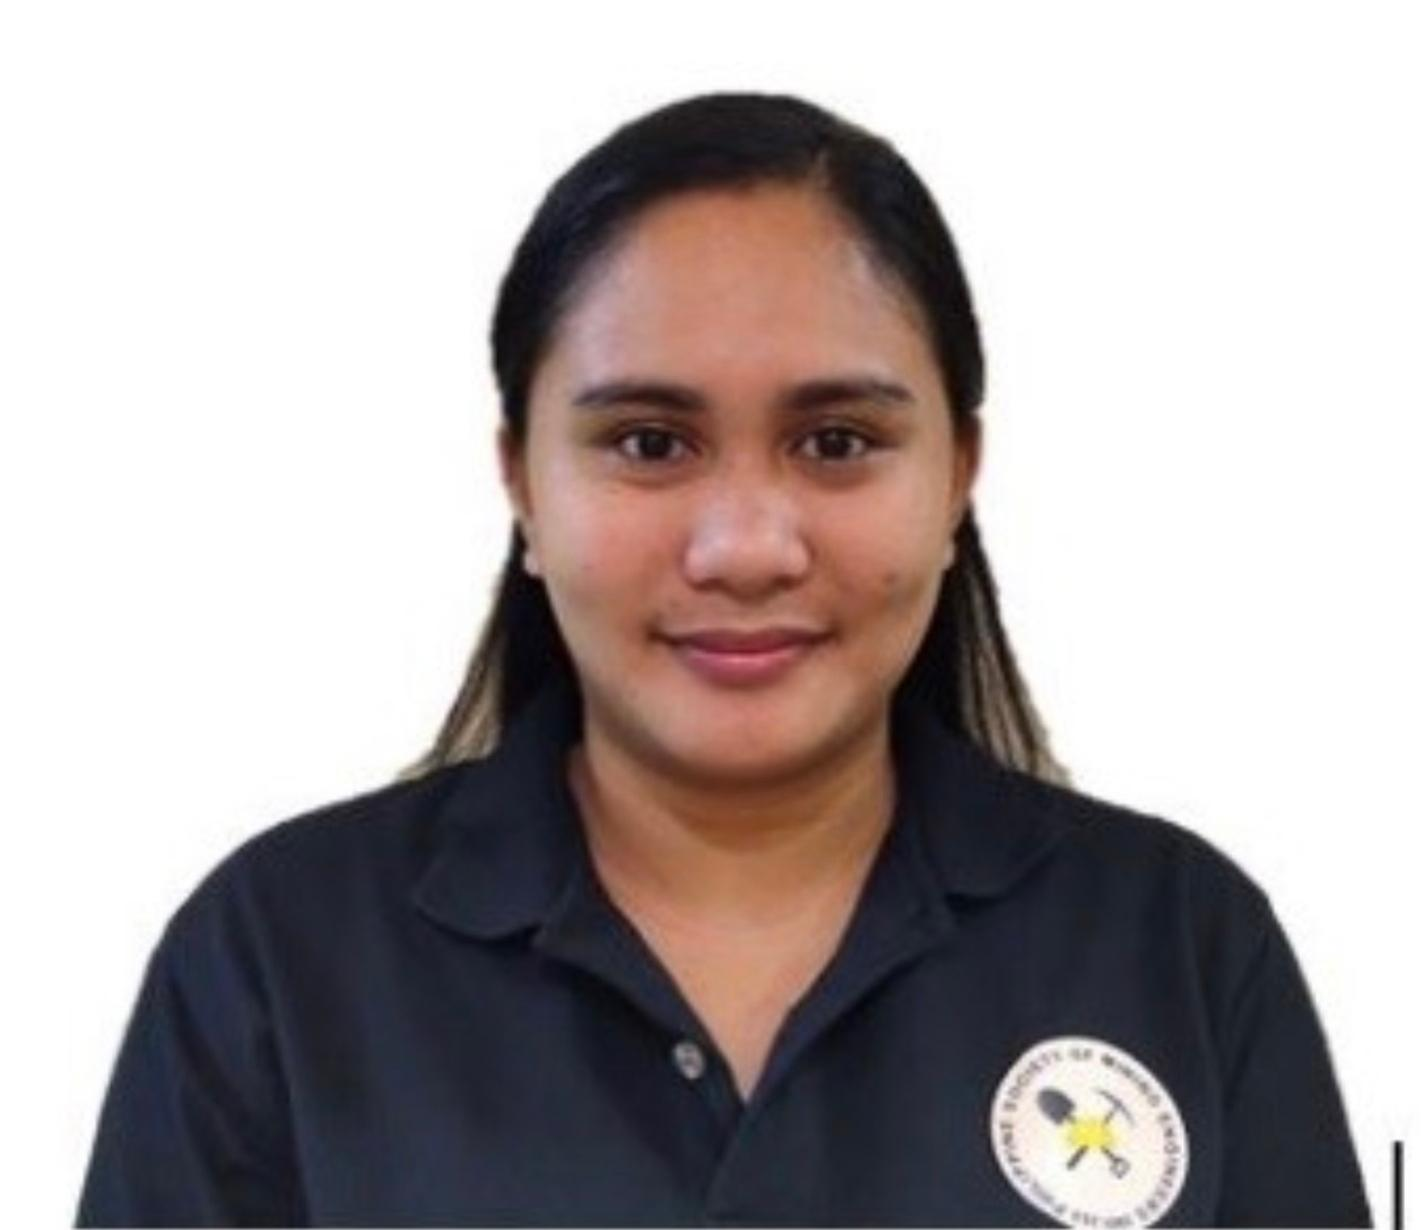
\includegraphics[width=1in]{img/burdeos}} \\ %TODO: Picture
    Bonbon, Butuan City, Agusan del Norte && \\
    melba.dominque@gmail.com && \\
\end{tabularx}

\vspace{20pt}

\textbf{PERSONAL INFORMATION}

\vspace{-10pt}
\hrulefill

\begin{tabular}{@{}l@{ : }l}
    DATE OF BIRTH & June 1, 1992 \\
    PLACE OF BIRTH & Butuan City \\
    AGE & 31 \\
    GENDER & Female \\
    NATIONALITY & Filipino \\
    RELIGION & Catholic \\
    CIVIL STATUS & Married \\
    FATHER'S NAME & Michael B. Burdeos \\
    MOTHER'S NAME & Josephine A. Burdeos \\
\end{tabular}

\vspace{20pt}

\textbf{EDUCATIONAL BACKGROUND}

\vspace{-10pt}
\hrulefill

\begin{tabular}{@{}l@{ : }l}
    COLLEGE & Saint Paul University Surigao \\
    & Corner Rizal and San Nicolas Streets, Surigao City \\
    HIGH SCHOOL & Agusan National High School\\
    & A.D. Curato St., Butuan City \\
    ELEMENTARY & La Trinidad Elementary School \\
    & Bonbon, Butuan City \\
\end{tabular}

\end{spacing}
\end{document}
